\textbf{Static Demand, Exact Solution}

The system risk constraint can be written
\begin{equation*} H(y) = \prod_{e \in \cE} \left( 1 - g_e(y_e) \right) \geq 1 - \epsilon
  \end{equation*}  
where $1 - g_e(y_e)$ is the probability that line $e$ doesn't fail given flow $y_e$, and taking the product of all these events gives the probability that no lines fail.  We have
\begin{align*}
  \ln \left( \prod_{e \in \cE}\left( 1 - g_e(y_e)\right) \right) &\geq \ln \left(  1 - \epsilon \right)  & g_e(y_e) \in [0,1) \forall e  \\
  \sum_{e \in \cE} \ln \left( 1-g_e(y_e) \right)  &\geq \ln \left( 1- \epsilon \right) & g_e(y_e) \in [0,1) \forall e 
\end{align*}
Letting $w_e = \ln \left( 1 -g_e(y_e) \right)$ take the value of a transformed line risk, we get our risk constraint
\begin{equation} \label{cceqn}
\sum_{e \in \cE} w_e \geq \ln \left( 1-\epsilon \right)
\end{equation}
with
\begin{align*}
w_e &= \ln \left( 1 - g_e(y_e)\right) \\
e^{w_e} &= 1-g_e(y_e) \\
g_e(x_e) + e^{w_e} &= 1 
\end{align*}
where $e^{w_e}$ is exponential function versus the subscript denoting the line.

And if we wanted to relax the constraint on $w_e$, we have $w_e \leq \ln \left( 1 - q_e(y_e) \right)$ since $w_e$ is related to the probability of success and lowering it would make it worse (and the real number would always satisfy the original constraint).
\begin{equation*}
g_e(y_e) + e^{w_e} \leq 1
\end{equation*}


\begin{figure}
\begin{center} 
\documentclass{standalone}
\usepackage{tikz}
\usepackage{pgfplots}
\begin{document}
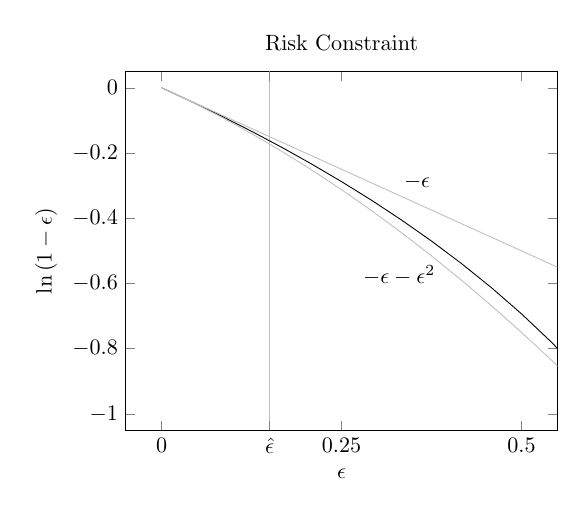
\begin{tikzpicture}[scale=.8]
\begin{axis}[ title=Risk Constraint,xlabel=$\epsilon$,ylabel=$\ln \left( 1-\epsilon \right)$,
  xmin=-.05,xmax=.55,
  ymin=-1.05,ymax=.05,
  xtick={0,.25,.5},
  	extra x ticks={.15},
	extra x tick style={grid=major},
	extra x tick labels={$\hat{\epsilon}$}
]
 \addplot[domain=0:.9999] { ln(1-x) };
 \addplot[domain=0:1,lightgray] {-x};
 \addplot[domain=0:1,lightgray] {-x - x^2};
  \node at (axis cs: .355,-.29) { $-\epsilon$};
  \node at (axis cs: .33,-.575) { $-\epsilon-\epsilon^2$};
\end{axis}
\end{tikzpicture}
\end{document}

\end{center}
\caption{Line risk substitution for individual branches}
\end{figure}
